\documentclass[9pt,landscape]{extarticle}
\usepackage[utf8]{inputenc}
\usepackage{multicol}
\usepackage{calc}
\usepackage[compact]{titlesec}
\usepackage{ifthen}
\usepackage[landscape]{geometry}
\usepackage{hyperref}
\usepackage{amsmath, amssymb, amsthm, bm, hyperref, float, mathtools}
% \usepackage{minted}
\usepackage{graphicx}
\usepackage{enumitem}
\usepackage{sectsty}

% Use images folder as root path for images
\graphicspath{{images/}}

% Remove extra spacing on bullet points
\setlist[itemize]{nosep, leftmargin=*}

% This sets page margins to .5 inch if using letter paper, and to 1cm
% if using A4 paper. (This probably isn't strictly necessary.)
% If using another size paper, use default 1cm margins.
\ifthenelse{\lengthtest { \paperwidth = 11in}}
    { \geometry{top=.5in,left=.5in,right=.5in,bottom=.5in} }
    {\ifthenelse{ \lengthtest{ \paperwidth = 297mm}}
        {\geometry{top=1cm,left=1cm,right=1cm,bottom=1cm} }
        {\geometry{top=1cm,left=1cm,right=1cm,bottom=1cm} }
    }

% Turn off header and footer
\pagestyle{empty}


% Redefine section commands to use less space
\makeatletter

\sectionfont{\normalsize}
\subsectionfont{\small}
\subsubsectionfont{\small}
\paragraphfont{\small}

\makeatother

% Define BibTeX command
\def\BibTeX{{\rm B\kern-.05em{\sc i\kern-.025em b}\kern-.08em
    T\kern-.1667em\lower.7ex\hbox{E}\kern-.125emX}}

% Don't print section numbers
\setcounter{secnumdepth}{0}

\setlength{\parindent}{0pt}
\setlength{\parskip}{0pt plus 0.5ex}

% -----------------------------------------------------------------------

\DeclarePairedDelimiter{\ceil}{\lceil}{\rceil}
\newcommand{\expect}[1]{\mathbf{E}[#1]}
\newcommand{\var}[1]{\text{Var(#1)}}
\newcommand{\cov}[1]{\text{Cov(#1)}}
\newcommand{\identity}{\mathbf{I}}
\newcommand*\diff{\mathop{}\!\mathrm{d}}
\newcommand*\Diff[1]{\mathop{}\!\mathrm{d^#1}}

% -----------------------------------------------------------------------

\begin{document}

\raggedright
\footnotesize
\begin{multicols}{3}

\setlength{\premulticols}{1pt}
\setlength{\postmulticols}{1pt}
\setlength{\multicolsep}{1pt}
\setlength{\columnsep}{2pt}

% =============================================================================

\section{Equations}

\textbf{Fourier transform}: $F(\omega) = \int_{-\infty}^{\infty} f(x) e^{-2\pi i \omega x} \diff x$ \\
\textbf{Inverse transform}: $f(x) = \int_{-\infty}^{\infty} F(\omega) e^{2\pi i \omega x} \diff\omega$ \\
\textbf{Euler's formula}: $e^{ix} = \cos x + i\sin x$ \\
\textbf{Poisson distribution}: $p(k; \lambda) = \frac{\lambda^k e^{-\lambda}}{k!}, \mu = \lambda, \sigma = \sqrt{\lambda}$ \\
\textbf{Convolution}: $(f * g)(x, y) = \sum_{i,j=-\infty}^{\infty}f(i, j)I(x-i, y-j)$ \\
\textbf{lerp}: $lerp(x, v_0, v_1) = v_0 + t(v_1 - v_0)$ \\
$\expect{X + c} = \expect{X} + c$ \\
$\expect{X + Y} = \expect{X} + \expect{Y}$ \\
$\expect{aX} = a\expect{X}$ \\
$\var{X} = \expect{X - \expect{X}^2} = \expect{x^2} - (\expect{x})^2$ \\
$\var{X + a} = \var{X}$ \\
$\var{aX} = a^2 \var{X}$ \\
$\var{aX + bY} = a^2 \var{X} + b^2 \var{Y} + 2ab \cov{X, Y}$ \\

% =============================================================================

\section{Rasterization}

\textbf{Antialiasing}: Removing frequencies above the Nyquist frequency (2 times the highest frequency) before sampling (Filtering before sampling) \\
\textbf{Line equation}: $L(x, y) = Ax + By + C$. On line: $L(x, y) = 0$, on right: $L(x, y) > 0$, on left: $L(x, y) < 0$. A point is inside a convex polygon if line tests for all lines (going clockwise) is greater than 0.

% =============================================================================

\section{Transforms}

\textbf{Transformation Order}:
\begin{itemize}[nosep]
    \item Object coordinates: Apply modeling transforms
    \item World (scene) coordinates: Apply viewing transform
    \item Camera (eye) coordinates: Apply perspective transform and homogeneous division
    \item Normalized device coordinates: Apply 2D screen transform
    \item Screen coordinates: Rasterization
\end{itemize}

\textbf{Homogeneous coordinates}: Points are defined as $(x, y, z, 1)$ and vectors by $(x, y, z, 0)$. \\

\textbf{Changing reference frame}: New coordinate frame defined by origin and coordinate axes:

\begin{multicols}{2}

Scaling

$$
\begin{bmatrix}
s & 0 & 0 \\
0 & s & 0 \\
0 & 0 & 1
\end{bmatrix}
$$

Rotation

$$
\begin{bmatrix}
\cos(\theta) & -\sin(\theta) & 0 \\
\sin(\theta) & \cos(\theta) & 0 \\
0 & 0 & 1
\end{bmatrix}
$$

\columnbreak

Translation

$$\begin{bmatrix}
1 & 0 & t_x \\
0 & 1 & t_y \\
0 & 0 & 1
\end{bmatrix}$$

Shear

$$
\begin{bmatrix}
1 & \lambda & 0 \\
0 & 1 & 0 \\
0 & 0 & 1
\end{bmatrix}
$$

\end{multicols}

Standard camera: Located at origin, pointing down negative z-axis, up vector is y axis. $r = v \times u$.

To standard camera (inverse)

$$
\begin{bmatrix}
r_x & r_y & r_z & 0 \\
u_x & u_y & u_z & 0 \\
-v_x & -v_y & -v_z & 0 \\
0 & 0 & 0 & 1
\end{bmatrix}
\begin{bmatrix}
1 & 0 & 0 & -e_x \\
0 & 1 & 0 & -e_y \\
0 & 0 & 1 & -e_z \\
0 & 0 & 0 & 1
\end{bmatrix}
$$

Rotation by angle $\alpha$ around axis $n$:

$$\cos(\alpha)\identity + (1 - \cos(\alpha))nn^T + \sin(\alpha)\begin{bmatrix}
    0 & n_z & -n_y \\
    -n_z & 0 & n_x \\
    n_y & -n_x & 0
\end{bmatrix}$$

\textbf{Hierarchical Transform}:

\textbf{Projective transform}: Project some point in the scene $(x, y, z)^T$ to a point on the image plane. If the center of projection is at $(0, 0, 0)^T$ and the image plane is at $z = d$, then $(x, y, z)^T \rightarrow (xd/z, yd/z, d)^T$.

Requires division by $z$, so use homogeneous coordinates:

$$
q = \begin{bmatrix}
        1 & 0 & 0 & 0 \\
        0 & 1 & 0 & 0 \\
        0 & 0 & 1 & 0 \\
        0 & 0 & 1/d & 0
    \end{bmatrix}
    \begin{bmatrix}
        x \\
        y \\
        z \\
        1
    \end{bmatrix} =
    \begin{bmatrix}
        xd/z \\
        yd/z \\
        d \\
        1
    \end{bmatrix}
$$


\textbf{Perspective projection}: parameterized by \textit{fovy}: vertical angular field of view, \textit{aspect}: width/height of field of view, \textit{near}: depth of near clipping plane, \textit{far}: depth of far clipping plane

Derived quantities: $top = near \cdot \tan(fovy)$, $bottom = -top$, $right = top \cdot aspect$, $left = -right$

Convert from camera coordinates to normalized device coordinates (NDC) by mapping the view volume frustum into a cube, where $(left, bottom, -near) \rightarrow (-1, -1, -1)$ and $(right, top, -far) \rightarrow (1, 1, 1)$. Linear transformation in homogeneous coordinates.

% $$\begin{bmatrix}
%     \frac{near}{right} & 0 & 0 & 0 \\
%     0 & \frac{near}{top} & 0 & 0 \\
%     0 & 0 & -\frac{far+near}{far-near} & \frac{-2(far\cdot near)}{far-near}\\
%     0 & 0 & -1 & 0
% \end{bmatrix}$$

% =============================================================================

\section{Geometry}

\textbf{Implicit geometry}: Surface defined where $f(x, y, z) = 0$. Can test if point is inside or outside easily, but hard to sample (what points lie on the surface?) Description can be compact, good for ray-to-surface intersections. No sampling error, easy to handle changes in topology. Hard to model complex shapes. \\
\textbf{Explicit geometry}: All points given directly, $f : \mathbb{R}^2 \rightarrow \mathbb{R}^3; (u, v) \rightarrow (x, y, z)$. Sampling easy, but hard to tell if point is inside/outside surface. \\
\textbf{Topological validity}: A 2D manifold is a surface that when cut with a sphere always yields a disk. Mesh manifolds always have the properties: edge connects two faces and two vertices, face consists of ring of edges and vertices, vertex consists of ring of edges and faces. $F - E + V = 2$ holds for a surface topologically equivalent to a sphere.

\begin{multicols}{2}
\begin{verbatim}
struct Halfedge {
    Halfedge *twin;
    Halfedge *next;
    Vertex *vertex;
    Edge *edge;
    Face *face; }
\end{verbatim}

\columnbreak

\begin{verbatim}
struct Vertex {
    Halfedge *halfedge; }
struct Edge {
    Halfedge *halfedge; }
struct Face {
    Halfedge *halfedge; }
\end{verbatim}
\end{multicols}

\textbf{Loop subdivision}: Split edges of original mesh in any order, then flip new edges that touch a new and old vertex.

\textbf{Catmull-Clark vertex update}: Converts an existing mesh to quads. Extraordinary points can increase during first iteration, but stays constant afterwards. Add a face point to the centroid of each face, add edge point (average of neighboring vertices and face points), connect face point to each edge point, update original points such that (n is valence of P, F is average of face points, R is average of edge points):

$$
P = \frac{F + 2R +(n-3)P}{n}
$$

\textbf{Barycentric Coordinates}: linearly interpolate values at vertices for a point in the triangle

$$(x, y) = \alpha A + \beta B + \gamma C$$
$$\alpha + \beta + \gamma = 1$$

\begin{multicols}{2}

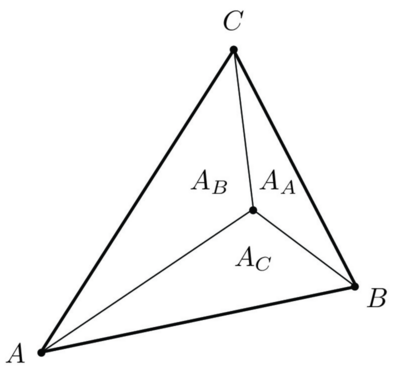
\includegraphics[scale=0.2]{barycentric_area}

\columnbreak

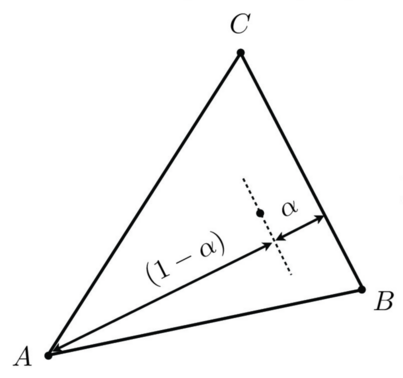
\includegraphics[scale=0.18]{barycentric_ratio}

\end{multicols}

\begin{align*}
\alpha &= \frac{-(x - x_B)(y_C - y_B) + (y - y_B)(x_C - x_B)}{-(x_A - x_B)(y_C - y_B) + (y_A - y_B)(x_C - x_B)} \\
\beta &= \frac{-(x - x_C)(y_A - y_C) + (y - y_C)(x_A - x_C)}{-(x_B - x_C)(y_A - y_C) + (y_B - y-C)(x_A - x_C)} \\
\gamma &= 1 - \alpha - \beta
\end{align*}

\begin{multicols}{3}
$\alpha = \frac{A_A}{A_A + A_B + A_C}$
\columnbreak
$\beta = \frac{A_B}{A_A + A_B + A_C}$
\columnbreak
$\gamma = \frac{A_C}{A_A + A_B + A_C}$
\end{multicols}

\textbf{Texture sampling}: Affine screen-space interpolation doesn't work, because linear interpolation in world coordinates yields nonlinear interpolation in screen coordinates. \textit{Magnification}: Each pixel is a small part of the texel. \textit{Minification}: each pixel includes many texels, leading to aliasing.

\textbf{Mipmaps}: Filter before sampling; use resolution that matches screen sampling rate. Estimate texture footprint using texture coordinates of neighboring screen samples, then use that to figure out which level of mipmap to use.

$$
D = \log_2 max\left(\sqrt{\left(\frac{du}{dx}\right)^2 + \left(\frac{dv}{dx}\right)^2}, \sqrt{\left(\frac{du}{dy}\right)^2 + \left(\frac{dv}{dy}\right)^2}\right)
$$

\textbf{Anisotropic filtering}: Mipmaps change depending on viewing angle. One way is to generate more mipmaps with variations on both $x$ and $y$, instead of just taking the max of both. Accomodation: Changes optical power to focus different distances. Vergence: rotation of eye in socket to ensure projection of object centered on retina

\textbf{Hermite matrix}:

\begin{align*}
    P(t) &= at^3 + bt^2 + ct + d \\
    &=  \begin{bmatrix}
            t^3 & t^2 & t & 1
        \end{bmatrix}
        \begin{bmatrix}
            2 & -2 & 1 & 1 \\
            -3 & 3 & -2 & -1 \\
            0 & 0 & 1 & 0 \\
            1 & 0 & 0 & 0
        \end{bmatrix}
        \begin{bmatrix}
            h_0 \\
            h_1 \\
            h_2 \\
            h_3
        \end{bmatrix} \\
    &= H_0(t)h_0 + H_1(t)h_1 + H_2(t)h_2 + H_3(t)h_3
\end{align*}

% \begin{align*}
%     H_0(t) &= 2t^3 - 3t^2 + 1 \\
%     H_1(t) &= -2t^3 + 3t^2 \\
%     H_2(t) &= t^3 - 2t^2 + t \\
%     H_3(t) &= t^3 - t^2
% \end{align*}

\textbf{Bezier Curves}

$$B_i^n(t) = \binom{n}{i} t^i (1-t)^{n-i}$$

\begin{align*}
    P(t) &= \sum_{i=0}^3 P_i B_i(t) \\
    &= (1-t)^3 P_0 + 3t(1-t)^2 P_1 + 3t^2(1-t) P_2 + t^3 P_3 \\
    &=  \begin{bmatrix}
            (1-t)^3 & 3t(1-t) & 3t^2(1-t) & t^3
        \end{bmatrix}
        \begin{bmatrix}
            P_0 \\
            P_1 \\
            P_2 \\
            P_3
        \end{bmatrix} \\
    &=  \begin{bmatrix}
            1 & t & t^2 & t^3
        \end{bmatrix}
        \begin{bmatrix}
            1 & 0 & 0 & 0 \\
            -3 & 3 & 0 & 0 \\
            3 & -6 & 3 & 0 \\
            -1 & 3 & -3 & 1
        \end{bmatrix}
        \begin{bmatrix}
            P_0 \\
            P_1 \\
            P_2 \\
            P_3
        \end{bmatrix}
\end{align*}

\textbf{de Casteljau Algorithm}:

\begin{align*}
B(t) &= (1-t)((1-t)P_0 + tP_1) + t((1-t)P_1 + tP_2) \\
&= (1-t)^2 P_0 + 2t(1-t)P_1 + t^2 P_3 \\
&=  \begin{bmatrix}
        (1-t)^2 & 2t(1-t) & t^2
    \end{bmatrix}
    \begin{bmatrix}
        P_0 \\
        P_1 \\
        P_2
    \end{bmatrix} \\
&=  \begin{bmatrix}
        1 & t & t^2
    \end{bmatrix}
    \begin{bmatrix}
        1 & 0 & 0 \\
        -2 & 2 & 0 \\
        1 & -2 & 1
    \end{bmatrix}
    \begin{bmatrix}
        P_0 \\
        P_1 \\
        P_2
    \end{bmatrix}
\end{align*}

$$b_{i,j}^{r,r} =
\begin{bmatrix}
    1 - u & u
\end{bmatrix}
\begin{bmatrix}
    b_{i, j}^{r-1, r-1} & b_{i, j+1}^{r-1, r-1} \\
    b_{i+1, j}^{r-1, r-1} & b_{i+1, j+1}^{r-1, r-1}
\end{bmatrix}
\begin{bmatrix}
    1 - v \\
    v
\end{bmatrix}$$

% =============================================================================

\section{Color/Radiometry}

\textbf{Solid angle}: $\Omega = \frac{A}{r^2}$, sphere has $4\pi$ steradians. $dA = (r d\theta)(r \sin\theta d\phi)$, $d\omega = \sin\theta d\theta d\phi$, $\Omega = \int_{S^2} d\omega = \int_0^{\phi} \int_0^{\theta} \sin\theta d\theta d\phi$. \\
\textbf{Radiant flux}: $\Phi \equiv \frac{dQ}{dt}$ [W] [lm], energy emitted over time (power) \\
\textbf{Radiant intensity}: $I(\omega) \equiv \frac{d\Phi}{d\omega}$ [$W/sr$] [$lm/sr=cd$], light emitted from a source, flux per unit solid angle \\
\textbf{Irradiance}: $E(x) \equiv \frac{d\Phi(x)}{dA}$ [$W/m^2$] [$lm/m^2=lux$], light falling on a surface, flux per unit area. Project area of object on unit sphere, project onto plane. \\
\textbf{Radiance}: $L(p, \omega) \equiv \frac{d^2\Phi(p, \omega)}{d\omega dA \cos\theta}$ [$W/(sr\cdot m^2)$] [$cd/m^2=lm/(sr\cdot m^2)=nit$], light travelling along a ray, flux per unit area per unit solid angle. Incident and exiting surface radiance are different (depends on material of surface)

\textbf{Lambert's cosine law}: Light per unit area is proportional to $\cos(\theta) = I \cdot n$, where $\theta$ is the angle between the normal and the light source and $I$ is a vector from hit point to light source.


% =============================================================================

\section{Rendering}

\textbf{Lambertian (Diffuse) shading}: Shading independent of view direction. $L_d = k_d (I / r^2) max(0, n\cdot l)$ \\
\textbf{Specular shading}: Close to mirror at the half-vector near normal. $h = \text{bisector}(v, l) = \frac{v + l}{\Vert v + l \Vert}$ \\
$L_s = k_s(I / r^2) \max(0, n \cdot h)^p$ \\
\textbf{Ambient shading}: doesn't depend on anything, adds constant color to account for disregarded illumination and fill in black shadows. Not physically accurate, since it's not based on any incoming radiance. $L_a = k_a I_a$

\textbf{Ray}: $r(t) = o + td, 0 \le t < \infty$ \\
\textbf{General implicit surface}: $p: f(p) = 0$ \\
\textbf{Substitute ray equation}: $f(o + td) = 0$ \\
\textbf{Sphere}: $(p - c)^2 - R^2 = 0$

$$t = \frac{(p - o) \cdot N}{d \cdot N} \rightarrow \frac{p_x - o_x}{d_x}$$

\textbf{Monte Carlo Integration}: $$F_N = \frac{1}{N} \sum_{i=1}^N \frac{f(x_i)}{p(x_i)}$$

\textbf{Inversion method}: Given $P(x) = Pr(X < x)$, solve for $x = P^{-1}(\xi)$. Need to know the integral of the PDF $p(x)$ for this to work. Example:

$$p_\lambda(x) = \lambda e^{-\lambda x}$$

$$\begin{aligned}
F(t) = P_\lambda(X \le t) &= \int_0^t \lambda e^{-\lambda x} dx \\
                          &= 1 - e^{-\lambda t}
\end{aligned}$$

$$F^{-1}(\xi) = \frac{-\log(1 - \xi)}{\lambda}$$

\textbf{Bidirectional Reflectance Distribution (BRDF)}: Non-negative (always returns a positive value for any input ray), respects linearity, reciprocity principle: $f_r(w_i \rightarrow w_r) = f_r(w_r \rightarrow w_i)$, conserves energy.

\textbf{Reflection equation}: $$
L_r(p, \omega_r) = \int_{H^2} f_r(p, \omega_i \rightarrow \omega_r) L_i(p, \omega_i) \cos \theta_i d\omega_i
$$ \\
\textbf{Transport function}: $tr(p, \omega)$ returns first surface intersection point in the scene along ray $(p, \omega)$ \\
\textbf{Radiance invariance}: $L_o(tr(p, \omega_i), -\omega_i) = L_i(p, \omega_i)$ \\
\textbf{Rendering equation}: $$
L_o(p, \omega_o) = L_e(p, \omega_o) + \int_{H^2} f_r(p, \omega_i \rightarrow \omega_o) L_o(tr(p, \omega_i), -\omega_i) \cos\theta_i d\omega_i
$$

% =============================================================================

\section{Animation}

\textbf{Inverse kinematics}: Solve for joint angles satisfying position of end-effector

\begin{align*}
\theta_2 &= \arccos\left(\frac{p_z^2 + p_x^2 - l_1^2 - l_2^2}{2l_1l_2}\right) \\
\theta_1 &= \frac{-p_zl_2\sin(\theta_2) + p_x(l_1 + l_2\cos(\theta_2))}{p_xl_2\sin(\theta_2) + p_z(l_1 + l_2\cos(\theta_2))}
\end{align*}

\textbf{Forward Euler}: $x(t + \Delta t) = x(t) + \Delta(t) \cdot v(x(t), t)$, $v(t + \Delta t) = v(t) + \Delta t \cdot f(x, v, t) / m$ \\
\textbf{Midpoint method}: $x_{mid} = x(t) + \Delta t / 2 \cdot v(x(t), t)$, $x(t + \Delta t) = x(t) + \Delta t \cdot v(x_{mid}, t)$ \\
\textbf{Implicit Euler}: $(t + \Delta t) = x(t) + \Delta(t) \cdot v(x(t + \Delta t), t)$ \\
\textbf{Adaptive step size}: Compute $x_T$, Euler step of size T. Computer $x_{T/2}$, two Euler steps of size T/2. Compute error, check if greater than threshold, reduce step size if necessary.


% =============================================================================

\section{Cameras}

\textbf{Exposure}: $H = T \times E$, exposure [controlled by shutter] = (time)(irradiance) [controlled by lens aperture and focal length] \\
\textbf{Aperture number (f-stop)}: $N = \frac{f}{D}$, focal length f, aperture diameter D. Irradiance proportional to square of D, inverse square f. Multiplying f-stop by $\sqrt{2}$ doubles exposure. Increasing 2 f-stops doubles depth of field. \\
\textbf{ISO (gain)}: multiply signal before analog/digital conversion. Linear effect: ISO 200 needs half as much light as ISO 100.

\textbf{Field of view}: $2\arctan(\frac{h}{2f})$, dependent on sensor size, focal length \\
\textbf{Depth of field}: aperture, focal length, object distance \\
\textbf{Exposure}: aperture, shutter, ISO \\
\textbf{Motion blur}: shutter \\
\textbf{Grain/noise}: ISO

\textbf{Phase-detection autofocus}: ray bundles from target object converge to points at different depths in camera depending on lens focus. Distance between phase-detect images correlates to distance in focus to target object.

\textbf{Lens maker's equation}: f, R1, R2 are signed, positive pointing to the right, radii point from surface to center

$$
\displaystyle\frac{1}{f} = \left(\frac{n_L}{n_A}-1\right)\left(\frac{1}{R_1}-\frac{1}{R_2}\right)
$$

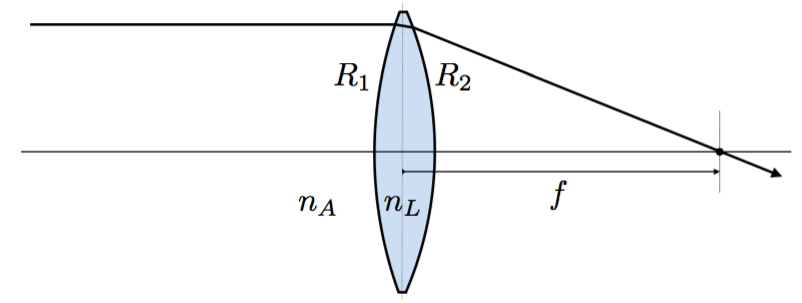
\includegraphics[scale=0.16]{lensmaker}

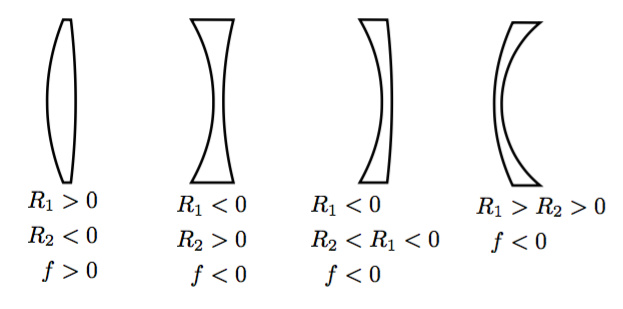
\includegraphics[scale=0.20]{lensmaker_radii}

\textbf{Gauss' ray-tracing construction}:

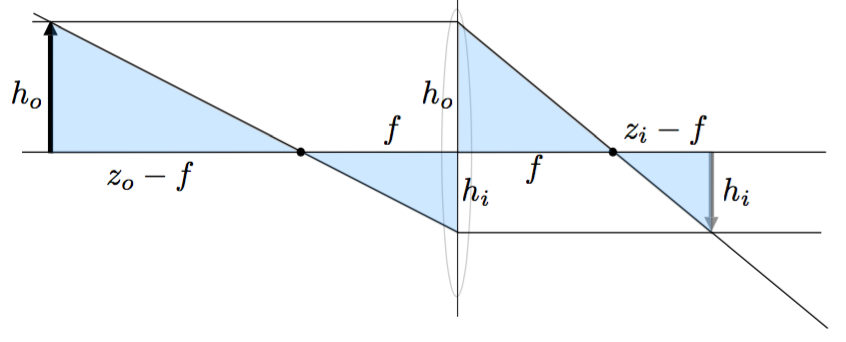
\includegraphics[scale=0.20]{gauss_ray}

\begin{multicols}{4}
$\frac{h_o}{z_o - f} = \frac{h_i}{f}$
\columnbreak
$\frac{h_o}{f} = \frac{h_i}{z_i-f}$
\columnbreak
$\frac{1}{f} = \frac{1}{z_i} + \frac{1}{z_o}$
\columnbreak
$m = \frac{h_i}{h_o} = \frac{z_i}{z_o}$
\end{multicols}

\textbf{Circle of confusion}

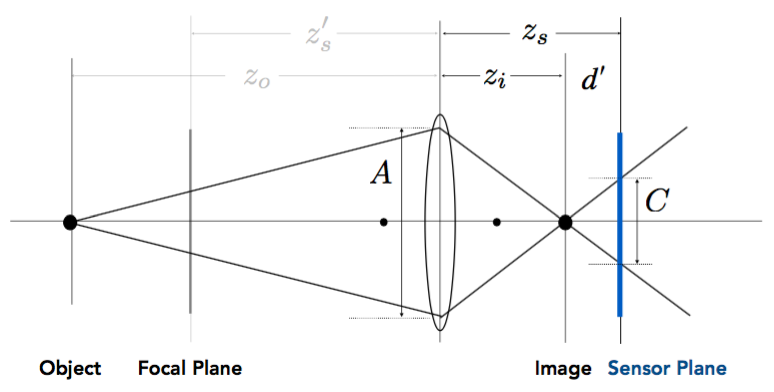
\includegraphics[scale=0.20]{circle_confusion}

$$
C = A\left(\frac{d^{\prime}}{z_i}\right) = A\frac{|z_s-z_i|}{z_i} = \frac{f}{N}\frac{|z_s-z_i|}{z_i}
$$

\textbf{Hyperfocal distance}: Maximizes depth of field (such that infinity is at limit of acceptable sharpness)

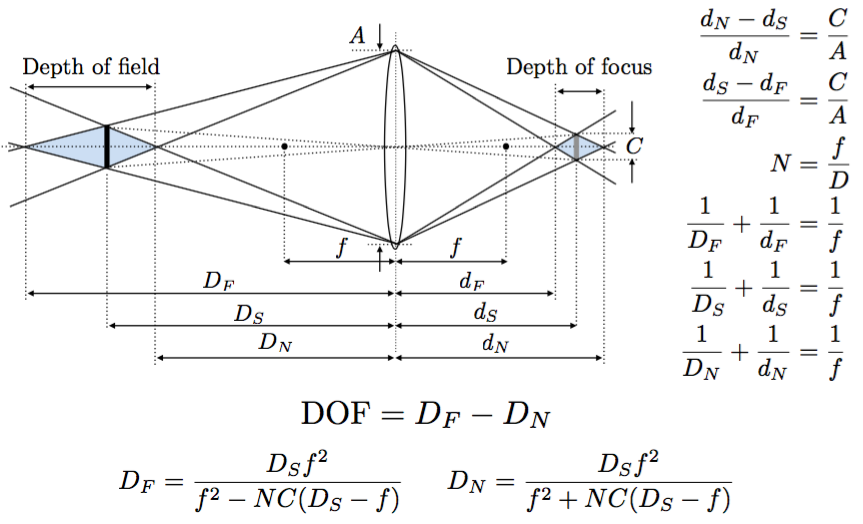
\includegraphics[scale=0.20]{dof}

\textbf{FSI vs BSI}: Back-side illuminated puts metal below diode below lens, whereas front-side illuminated puts metal in-between lens and diode. BSI makes more light hit the diode (doesn't have to make it through a tunnel of metal). \\
\textbf{Signal-to-noise (SNR)}: $\frac{\mu}{\sigma} = \frac{\lambda}{\sqrt{\lambda}} = \sqrt{\lambda}$

\textbf{Light-field camera}: Uses radiance flowing along every ray (4D) rather than irradiance at every pixel on plane (2D). Microlenses cover multiple pixels. Light-field data preserves directional intensity information, provides flexibility over focus/aberrations

\textbf{VR displays}: Add stereo (different left/right eye views), parallax (different views as user moves)

% =============================================================================

% \section{Image Processing}
%
% \textbf{JPEG compression}: Uses Y'CbCr color space (luma, blue-yellow and red-green). Subsample chroma channels, luma stays same. Uses discrete cosine transform (DCT), prioritizes low frequencies
%
% \textbf{Sobel edge detection}: Find pixels with large gradients $G = \sqrt{G_x^2 + G_y^2}$
%
% \begin{multicols}{2}
% Horizontal gradients
%
% $$
% G_x = \begin{bmatrix}
% -1 & 0 & 1 \\
% -2 & 0 & 2 \\
% -1 & 0 & 1
% \end{bmatrix} * I
% $$
%
% \columnbreak
%
% Vertical gradients
%
% $$
% G_y = \begin{bmatrix}
% -1 & -2 & -1 \\
% 0 & 0 & 0 \\
% 1 & 2 & 1
% \end{bmatrix} * I
% $$
% \end{multicols}

% =============================================================================

\end{multicols}
\end{document}
